\documentclass{report}
\usepackage[spanish]{babel}
\usepackage[utf8]{inputenc}
\usepackage{graphicx, longtable, float, titlesec, hyperref, enumitem, dingbat, multicol}
\usepackage[dvipsnames]{xcolor}
\usepackage[margin=2.75cm]{geometry}

\hypersetup{
    hidelinks = true
}

\titleformat{\chapter}[display]
  {\normalfont\bfseries}{}{0pt}{\Huge\thechapter.\space}

\titleformat{name=\chapter,numberless}[display]
  {\normalfont\bfseries}{}{0pt}{\Huge}

\titlespacing*{\chapter}{0pt}{-50pt}{20pt}

\begin{document}
    \begin{titlepage}
        \centering
        
\includegraphics[width=0.6\textwidth]{./img/logo.jpg}\\
        \vspace{1cm}
        \LARGE Software de Gestión de Empresa\\
        \vspace{0.5cm}
        \Large Ingeniería Informática de Gestión y Sistemas de Información\\
        \vspace{3cm}
        \Huge Proyecto de la asignatura\\
        \huge SoloG\\
        \vspace{2.5cm}
        \Large Autores:\\
        \vspace{0.2cm}
        \large Xabier Gabiña\\
        \large Ibai Sologuestoa\\
        \large Asier Cardoso\\
        \large Leire Becerra\\
        \large Adair Gondan\\
        \vfill
        \today
    \end{titlepage}
    \tableofcontents
    \listoffigures
    \listoftables
    \chapter{Análisis del sector}
      \paragraph*{}{El sector industrial de la videovigilancia es una parte de la industria de la seguridad y la tecnología. Se encarga de proporcionar sistemas de vigilancia visual para una amplia gama de aplicaciones en entornos industriales y domesticos, como fábricas, almacenes, instalaciones de energía, plantas de producción, hogares, entre otros.}
      \section{Productos ofertados}
        \paragraph*{}
        {
          Los productos ofertados en el sector de la videovigilancia son muy variados y se pueden clasificar en diferentes categorías. Algunos de los productos más comunes son: \cite{wiki-videovigilancia-ip}
        }
        \begin{multicols}{2}
          \begin{itemize}
            \item Cámaras de video
            \item Grabador de vídeo 
            \item Video Server Encoder
            \item Software de análisis de vídeo
            \item Dispositivos de visualización
            \item LED infrarrojos
            \item Sensores
            \item Reconocimiento Facial
          \end{itemize}
        \end{multicols}
        
      \section{Mercado objetivo}
        \paragraph*{}
        {
          El mercado objetivo de la videovigilancia es muy amplio y abarca desde la empresa hasta el hogar. 
          Aun así, el mayor volumen de ventas se da en el sector empresarial, donde se requieren sistemas de videovigilancia para proteger las instalaciones, controlar el acceso de personal y vehículos, y prevenir robos y actos vandálicos.
          Dentro del sector empresarial, se ha registrado un aumento en la demanda de sistemas de videovigilancia en el segmento de \textbf{infraestructuras críticas}, como aeropuertos, estaciones de tren, puertos, centrales eléctricas, entre otros.\cite{mordor-video-surveillance}
        }
        \paragraph*{}
        {
          Hay que tambien tener en cuenta que la demanda no es la misma en todos los países. La videovigilancia tiene un mayor peso en países como \textbf{Estados Unidos}, \textbf{China}, \textbf{Reino Unido}, \textbf{India} y \textbf{Brasil}, donde se han registrado un mayor número de instalaciones de sistemas de videovigilancia.\cite{mordor-video-surveillance}
        }
        \paragraph*{}
        {
          Tambien se espera que \textbf{Asia Pacífico} sea la región con mayor crecimiento en el mercado de la videovigilancia en los próximos años, debido al concepto de ciudades inteligentes ampliamente extendido especialmente en \textbf{China} y la creciente urbanización en la región.\cite{mordor-video-surveillance}
        }
        \begin{figure}[H]
          \centering
          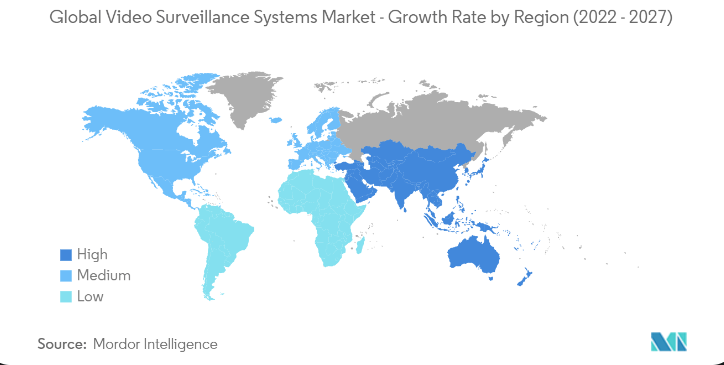
\includegraphics[width=0.7\textwidth]{./img/ssm.png}
          \caption{Mercado de la videovigilancia en 2022-2027}
        \end{figure}
      \section{Materias primas}
        \paragraph*{}{Las materias primas necesarias para la fabricación de los productos de videovigilancia son muchas y muy variadas. Algunas de las materias primas más usadas son:}
        \begin{multicols}{2}
          \begin{itemize}
            \item Plástico
            \item Metal
            \item Cables
            \item Circuitos integrados
            \item Lentes
            \item Sensores
            \item LED
            \item Software
          \end{itemize}
        \end{multicols}
      \section{Proveedores}
        \paragraph*{}
        {
          Los proveedores de materias para la fabricación de productos de videovigilancia se pueden clasificar en dos categorías, proveedores de componentes electrónicos y proveedores de software. 
          Algunos de los proveedores más importantes de componentes electrónicos son \textbf{Canon}, \textbf{Axis}, \textbf{Milestone} y \textbf{BCD}. 
          Algunos de los proveedores más importantes de software son \textbf{EarthCam} e \textbf{Infotech}
        }
      \section{Cinco fuerzas de Porter}
        \subsection*{Rivalidad entre competidores existentes}
          \paragraph*{}{El mercado de la videovigilancia es muy competitivo, con un gran número de empresas que ofrecen productos y servicios similares. La rivalidad entre competidores existentes es alta, lo que significa que las empresas deben competir en precio, calidad, innovación y servicio al cliente para mantener o aumentar su cuota de mercado.}
        \subsection*{Amenaza de productos sustitutos}
          \paragraph*{}{La amenaza de productos sustitutos en el mercado de la videovigilancia es baja, ya que los sistemas de videovigilancia son una parte esencial de la seguridad en muchos entornos, como empresas, hogares, infraestructuras críticas, entre otros.}
        \subsection*{Amenaza de productos o servicios sustitutos}
          \paragraph*{}{La amenaza de productos o servicios sustitutos en el mercado de la videovigilancia es baja, ya que los sistemas de videovigilancia son una parte esencial de la seguridad en muchos entornos, como empresas, hogares, infraestructuras críticas, entre otros.}
        \subsection*{Poder de negociación de los compradores}
          \paragraph*{}{El poder de negociación de los compradores en el mercado de la videovigilancia es alto, ya que los compradores tienen una amplia gama de opciones para elegir y pueden comparar precios, calidad, innovación y servicio al cliente antes de tomar una decisión de compra.}
        \subsection*{Poder de negociación de los proveedores}
          \paragraph*{}{El poder de negociación de los proveedores en el mercado de la videovigilancia es bajo, ya que hay muchos proveedores de componentes electrónicos y software que compiten por el negocio de las empresas de videovigilancia.}
      \section{Competidores}
        \paragraph*{}{Debido a que el mercado de la videovigilancia se actualiza constantemente los actores del mercado fluctuan mucho y son altamente competitivos. Los competidores más importantes en el mercado de la videovigilancia son:}
        \begin{multicols}{3}
          \begin{itemize}
            \item Axis Communications AB
            \item Bosch Security Systems Incorporated
            \item Honeywell Security Group
            \item Samsung Group
            \item Panasonic Corporation
            \item Schneider Electric SE
          \end{itemize}
        \end{multicols}
        \paragraph*{}{Como hemos comentado, el mercado de la videovigilancia es muy competitivo, lo que significa que \textbf{no es un mercado consolidado} por lo que se podria llegar a entrar y competir en el con una buena estrategia.}
        \begin{figure}[H]
          \centering
          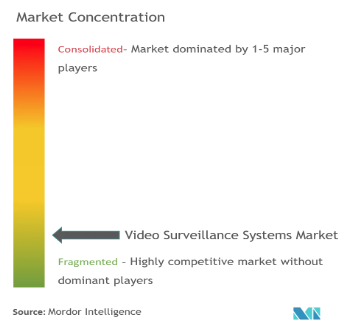
\includegraphics[width=0.4\textwidth]{./img/competidores.png}
          \caption{Competidores en el mercado de la videovigilancia}
        \end{figure}
    \chapter{Diseño del sistema de gestión}
        \section{Estructura empresarial}
          \paragraph*{}{
            La estructura empresarial es el marco que define cómo se dividen, agrupan y coordinan las actividades dentro de una empresa u organización. 
            Esta estructura establece la jerarquía de autoridad, las relaciones de supervisión, los flujos de comunicación y las responsabilidades de cada unidad dentro de la organización.
          }
          \paragraph*{}
          {
            Una estructura organizativa eficaz ayuda a clarificar las funciones de cada departamento y puesto de trabajo, facilita la coordinación entre diferentes áreas, promueve la eficiencia operativa y favorece el logro de los objetivos organizacionales.
          }
          \paragraph*{}
          {
            La estructura de SoloG es una estructura jerarquica, con una clara división de departamentos y niveles de decisión:
          }
          \subsection{Dirección General}
            \begin{itemize}
            \item Director General - Responsable de la visión estratégica de la empresa, toma de decisiones clave y supervisión general de todas las operaciones.
            \end{itemize}
          \subsection{Departamento Administrativo y Financiero}
            \begin{itemize}
            \item Director Administrativo y Financiero - Encargado de la gestión financiera, contabilidad, presupuestos, nóminas, y gestión de recursos humanos.
            \item Contadores y Analistas Financieros - Encargados de la contabilidad detallada, análisis financiero y reportes.
            \item Recursos Humanos - Responsable de la contratación, capacitación, evaluación del desempeño y gestión de beneficios de los empleados.
            \end{itemize}
          \subsection{Departamento Comercial y Marketing}
            \begin{itemize}
            \item Director Comercial y de Marketing - Encargado de desarrollar estrategias de ventas, mercadotecnia, publicidad y relaciones públicas.
            \item Ejecutivos de Ventas - Responsables de la identificación de clientes potenciales, negociación de contratos y cierre de ventas.
            \item Especialistas en Marketing Digital - Encargados de la presencia en línea, publicidad en redes sociales, SEO y marketing de contenidos.
            \end{itemize}
          \subsection{Departamento de Operaciones}
            \begin{itemize}
            \item Director de Operaciones - Encargado de la logística, implementación de sistemas de videovigilancia, y gestión de proyectos.
            \item Ingenieros de Sistemas de Videovigilancia - Responsables del diseño, instalación y mantenimiento de sistemas de seguridad.
            \item Técnicos de Campo - Encargados de la instalación, mantenimiento preventivo y reparación de equipos de videovigilancia.
            \end{itemize}
          \subsection{Departamento de Servicio al Cliente}
            \begin{itemize}
            \item Director de Servicio al Cliente - Responsable de garantizar la satisfacción del cliente, resolver quejas y problemas, y mantener relaciones positivas con los clientes.
            \item Representantes de Servicio al Cliente - Encargados de atender consultas, proporcionar soporte técnico y asistencia postventa.
            \end{itemize}
          \subsection{Departamento de Desarrollo Tecnológico}
            \begin{itemize}
            \item Director de Desarrollo Tecnológico - Encargado de la investigación y desarrollo de nuevas tecnologías en videovigilancia.
            \item Ingenieros de Software y Hardware - Responsables del desarrollo de software de vigilancia, firmware y hardware especializado.
            \end{itemize}
          \subsection{Departamento Legal y de Cumplimiento}
            \begin{itemize}
            \item Director Legal y de Cumplimiento - Encargado de garantizar que la empresa cumpla con todas las regulaciones legales y normativas relacionadas con la videovigilancia.
            \item Abogados y Asesores Legales - Responsables de la redacción de contratos, gestión de litigios y asesoramiento legal.
            \end{itemize}
        \clearpage\section{Procesos}
          \paragraph*{}
          {
            Los procesos son las actividades y tareas que se realizan en una empresa para lograr los objetivos organizacionales. 
            Son esenciales para la operación eficiente y efectiva de una empresa, ya que definen cómo se llevan a cabo las actividades, cómo se asignan los recursos y cómo se logran los resultados.
          }
          \paragraph*{}
          {
            Los procesos de SoloG se pueden clasificar en diferentes categorías:
          }
          \subsection{Procesos de Ventas y Marketing}
            \begin{itemize}
              \item Identificación de Clientes Potenciales - Identificar empresas y organizaciones que puedan necesitar sistemas de videovigilancia.
              \item Desarrollo de Estrategias de Ventas - Crear estrategias de ventas personalizadas para cada cliente potencial.
              \item Negociación de Contratos - Negociar los términos y condiciones de los contratos con los clientes.
              \item Cierre de Ventas - Cerrar acuerdos de venta y asegurar la satisfacción del cliente.
              \item Desarrollo de Estrategias de Marketing - Crear campañas de marketing para promocionar los productos y servicios de la empresa.
              \item Publicidad y Promoción - Publicar anuncios en línea, en medios impresos y en eventos para promocionar la empresa.
              \item Relaciones Públicas - Mantener relaciones positivas con los medios de comunicación, clientes y la comunidad.
            \end{itemize}
          \subsection{Procesos de Diseño y Consultoria}
            \begin{itemize}
              \item Diseño de Sistemas de Videovigilancia - Diseñar sistemas de videovigilancia personalizados para las necesidades de cada cliente.
              \item Consultoría en Seguridad - Asesorar a los clientes sobre las mejores prácticas de seguridad y las soluciones más efectivas.
              \item Evaluación de Riesgos - Evaluar los riesgos de seguridad de las instalaciones de los clientes y recomendar soluciones.
              \item Implementación de Sistemas de Seguridad - Instalar y configurar sistemas de videovigilancia en las instalaciones de los clientes.
              \item Capacitación de Personal - Capacitar al personal de los clientes en el uso de los sistemas de videovigilancia.
            \end{itemize}
          \subsection{Procesos de Instalación y Mantenimiento}
            \begin{itemize}
              \item Instalación de Equipos de Videovigilancia - Instalar cámaras, grabadores de video y otros equipos de videovigilancia en las instalaciones de los clientes.
              \item Configuración de Sistemas de Seguridad - Configurar los sistemas de videovigilancia para garantizar su funcionamiento óptimo.
              \item Mantenimiento Preventivo - Realizar inspecciones regulares y mantenimiento preventivo de los sistemas de videovigilancia.
              \item Reparación de Equipos - Reparar equipos de videovigilancia dañados o defectuosos.
              \item Actualización de Software y Firmware - Actualizar el software y firmware de los sistemas de videovigilancia para garantizar su seguridad y eficacia.
            \end{itemize}
          \subsection{Procesos de Servicio al Cliente}
            \begin{itemize}
              \item Atención de Consultas - Atender consultas de los clientes sobre productos, servicios y precios.
              \item Soporte Técnico - Proporcionar asistencia técnica a los clientes para resolver problemas con los sistemas de videovigilancia.
              \item Asistencia Postventa - Brindar asistencia a los clientes después de la venta para garantizar su satisfacción.
              \item Resolución de Quejas y Problemas - Resolver quejas y problemas de los clientes de manera rápida y eficaz.
              \item Mantenimiento de Relaciones con Clientes - Mantener relaciones positivas con los clientes para fomentar la lealtad y la satisfacción.
            \end{itemize}
          \subsection{Procesos de Investigación y Desarrollo}
            \begin{itemize}
              \item Investigación de Nuevas Tecnologías - Investigar y evaluar nuevas tecnologías en videovigilancia para mejorar los productos y servicios de la empresa.
              \item Desarrollo de Software de Videovigilancia - Desarrollar software especializado para la gestión y análisis de sistemas de videovigilancia.
              \item Desarrollo de Hardware Especializado - Diseñar y fabricar hardware especializado para sistemas de videovigilancia.
              \item Pruebas y Validación de Productos - Realizar pruebas exhaustivas y validación de productos antes de su lanzamiento al mercado.
              \item Implementación de Mejoras - Implementar mejoras continuas en los productos y servicios de la empresa para mantenerse a la vanguardia de la tecnología.
            \end{itemize}
        \clearpage\section{Productos}
          \subsection{Cámaras de Seguridad}
            \begin{itemize}
              \item Cámaras de CCTV (circuito cerrado de televisión) para interior y exterior.
              \item Cámaras domo, tipo bala, PTZ (pan-tilt-zoom) y de tipo discreto.
              \item Cámaras con tecnología de visión nocturna (infrarroja) para grabación en condiciones de poca luz.
              \item Cámaras con resolución de alta definición (HD) y ultra alta definición (4K) para imágenes claras y detalladas.
            \end{itemize}
          \subsection{Sistemas de Grabación}
            \begin{itemize}
              \item Grabadoras de vídeo digital (DVR) y grabadoras de vídeo en red (NVR) para almacenamiento y gestión de grabaciones.
              \item Almacenamiento en disco duro con capacidades variables para retención de datos a largo plazo.
              \item Sistemas de almacenamiento en la nube para copias de seguridad y acceso remoto a grabaciones.
            \end{itemize}
          \subsection{Sistemas de Control de Acceso}
            \begin{itemize}
              \item Lectores de tarjetas de acceso, teclados numéricos y sistemas biométricos de reconocimiento.
              \item Cerraduras electrónicas y electromagnéticas para control de puertas.
              \item Software de gestión de acceso para administrar usuarios, horarios y permisos de acceso.
            \end{itemize}
          \subsection{Sistemas de Alarma}
            \begin{itemize}
              \item Sensores de movimiento, sensores de puertas y ventanas, y detectores de humo.
              \item Sirenas y luces estroboscópicas para disuadir intrusos y alertar a los ocupantes.
              \item Paneles de control centralizados para armar, desarmar y gestionar alarmas.
            \end{itemize}
          \subsection{Sistemas de Monitoreo Remoto}
            \begin{itemize}
              \item Aplicaciones móviles y software de escritorio para visualizar y controlar sistemas de videovigilancia desde cualquier ubicación.
              \item Servicios de monitoreo remoto por parte de personal de seguridad o centro de monitoreo externo.
            \end{itemize}
        \clearpage\section{Servicios}
          \subsection{Consultoría en Seguridad}
            \begin{itemize}
              \item Evaluación de riesgos de seguridad y recomendaciones para mejorar la protección de las instalaciones.
              \item Desarrollo de planes de seguridad y políticas de gestión de riesgos.
            \end{itemize}
          \subsection{Diseño e Instalación de Sistemas}
            \begin{itemize}
              \item Planificación y diseño de sistemas de videovigilancia personalizados según las necesidades y el entorno del cliente.
              \item Instalación profesional de equipos de seguridad, incluyendo cableado, montaje y configuración de dispositivos.
            \end{itemize}
          \subsection{Mantenimiento Preventivo y Soporte Técnico}
            \begin{itemize}
              \item Programación de visitas periódicas para inspección y mantenimiento de equipos.
              \item Soporte técnico remoto y en sitio para resolver problemas y asegurar el funcionamiento continuo del sistema.
            \end{itemize}
          \subsection{Capacitación y Formación}
            \begin{itemize}
              \item Entrenamiento para usuarios finales en el manejo y operación del sistema de videovigilancia.
              \item Capacitación técnica para personal de seguridad y administradores del sistema.
            \end{itemize}
          \subsection{Servicios de Monitoreo y Respuesta a Alarmas}
            \begin{itemize}
              \item Monitoreo en tiempo real de cámaras y sistemas de seguridad por parte de personal capacitado.
              \item Respuesta a eventos de alarma, incluyendo notificación a las autoridades pertinentes según sea necesario.
            \end{itemize}
    \chapter{Implementación de la solución}
    \chapter{Presentación de los resultados}
    \bibliographystyle{plain}
    \bibliography{bibliografia.bib}
\end{document}